\documentclass[12pt, a4paper]{article}
\usepackage[utf8]{inputenc}
\usepackage{amsmath} 
\usepackage{amssymb}
\usepackage{listings}
\usepackage{graphicx}
\usepackage{float}
\usepackage[dvipsnames]{xcolor}
\PassOptionsToPackage{hyphens}{url}
\usepackage{hyperref}

\begin{document}

\section{Design}

\subsection{Data Collection}

\texttt{get\_valid\_stop\_ids} is called once a week to obtain a list of valid stop ids and this list of valid stop ids along with their common English name is stored in a database for each route. \\

The over arching algorithm for collecting data is shown in Figure \ref{fig:main-flow}. For each bus route the following steps occur. \\

\begin{figure}[H]
\begin{center}
    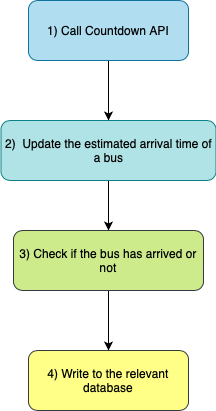
\includegraphics[keepaspectratio, width=5cm]{Images/Data-Collection-new-overarch.png}
    \caption{Overarching data collection algorithm}
    \label{fig:main-flow}
\end{center}
\end{figure}

\subsubsection{Technology Choices}

The code that performs the API calls and logic for whether a bus has arrived or not is written in Python. \\

Initially, the code was hosted on AWS, using AWS Lambdas to run the data collection functionality and AWS DynamoDB to store the data. I chose AWS because its free tier had generous WORD I CANT THINK OF RIGHT NOW and it already had the features that I wanted as part of my data collection algorithm built in. i.e. i didn't have to set up a server, it would do the hosting for me, linking dynamodb and lambdas was really easy because they were built to be run together. unfortunately exceeded free tier and also when i began doing the data analytics, found having a relational database made life easier for querying because dynamodb is nosql so key-value pair. \\

A PostgreSQL database is used to store all of the tables. PostgreSQL was chosen because \\

Python, Docker containers, Postgresql, DoC Cloud VM

\clearpage

\end{document}